\chapter{Literature Review}

To have a better understanding of the project, it is important to review the literature on the topic.\\
In particular, we decided to analyze an article extracted from the 2020 International Conference on Data Science, Artificial Intelligence, and Business Analytics (DATABIA). The article is titled "Predicting a Hit Song with Machine Learning: Is there an apriori secret formula?" by authors: A. H. Raza and K. Nanath. \\
The authors collected data from the Billboard Hot 100 Charts from 2017 to 2019, and they classified a song as Hit when it appeared in the top 20 at the end of each month, as a Non-Hit if it was amongst the bottom ten songs at the end of each month.
This different approach of collecting data allowed the authors to have a better composition of Hit songs vs Non-Hit songs (337 vs 310). To collect the audio features, they also used a Spotify API. The audio features collected were the same as in our dataset. \\
The authors used also the lyrics of the songs to extract the sentiment analysis. This showed that the sentiment of the lyrics of the Hit songs was in general more positive than the sentiment of the lyrics of the Non-Hit songs, but there wasn't a huge difference. The authors concluded that the sentiment analysis of the lyrics of the songs didn't have a significant impact on the prediction of the popularity of the songs. \\
They didn't study popularity of the songs across different regions, but they used the same approach to predict the popularity of the songs: they used Logistic Regression, Decision Tree, Random Forests and Naïve Bayes.
The algorithm with the highest accuracy was Logistic Regression at 52.0\%. \\
The authors discovered that Danceability was one of the most significant features, if not the most significant. Other features that proved to be significant were Energy, Valence, Tempo, Speechiness, and Loudness. At the same time the algorithms accuracy wasn't so high, which made it difficult to predict if a song will be popular or not with precision. \\

\begin{figure} [H]
    \centering
    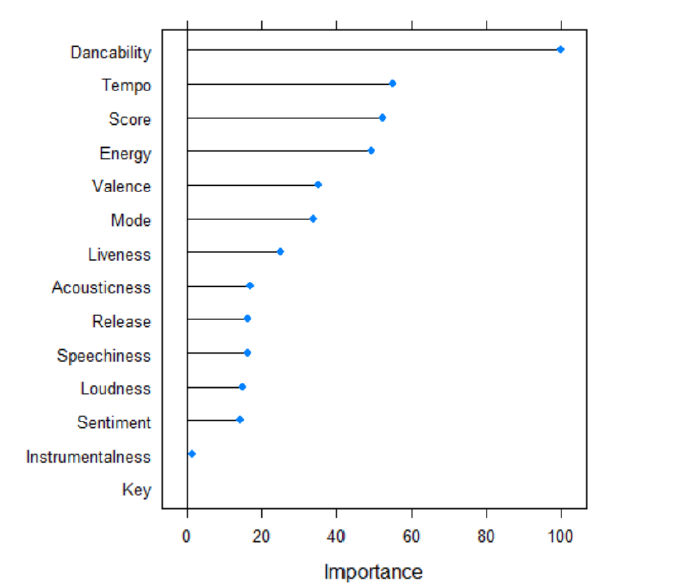
\includegraphics[width=0.5\textwidth]{media/state_of_art_feat_imp.png}
    \caption{Feature Importance}
    \label{fig:feature_importance}
\end{figure}